\documentclass[aspectratio=169,10pt]{beamer}

\usepackage[utf8]{inputenc}
\usepackage[T1]{fontenc}
\usepackage[spanish,es-tabla]{babel}
\usepackage{graphicx}
\usepackage{booktabs}
\usepackage{array}
\usepackage{multicol}
\usepackage{amsmath}
\usepackage{pgfpages}
\usepackage{xcolor}
\usepackage{tikz}
\usetikzlibrary{arrows.meta,positioning,fit,calc,shapes.geometric,decorations.pathreplacing}
\usepackage{hyperref}

% Para imprimir las notas del presentador, cambiar a:
% \setbeameroption{show notes on second screen=right}
\setbeameroption{hide notes}

\graphicspath{{../memoria/imagenes/}{../memoria/figuras/}{assets/}{imagenes/}}

\usetheme{Madrid}
\usecolortheme{default}
\setbeamertemplate{navigation symbols}{}
\setbeamertemplate{caption}[numbered]
\setbeamerfont{title}{size=\Large,series=\bfseries}
\setbeamerfont{frametitle}{size=\large,series=\bfseries}

\definecolor{deepgreen}{HTML}{0B3D2E}
\definecolor{accent}{HTML}{E76F51}
\definecolor{soft}{HTML}{F1FAEE}
\definecolor{greenish}{HTML}{2A9D8F}
\definecolor{warning}{HTML}{F4A261}
\definecolor{muted}{HTML}{6C757D}
\definecolor{lightgray}{HTML}{F6F7F8}

\definecolor{tfmgreen}{HTML}{0B4A36}
\definecolor{softgreen}{HTML}{EAF5F0}
\definecolor{softred}{HTML}{F9D6CA}
\definecolor{softblue}{HTML}{DDEAF7}
\definecolor{softyellow}{HTML}{FFF0C7}
\definecolor{linegray}{HTML}{6E7D77}

\setbeamercolor{structure}{fg=deepgreen}
\setbeamercolor{palette primary}{fg=white,bg=deepgreen}
\setbeamercolor{palette secondary}{fg=white,bg=deepgreen!85!black}
\setbeamercolor{palette tertiary}{fg=white,bg=deepgreen!70!black}
\setbeamercolor{frametitle}{fg=white,bg=deepgreen}
\setbeamercolor{title}{fg=white,bg=deepgreen}
\setbeamercolor{subtitle}{fg=white}
\setbeamercolor{author}{fg=white}
\setbeamercolor{institute}{fg=white}
\setbeamercolor{date}{fg=white}
\setbeamercolor{title page}{fg=white,bg=deepgreen}
\setbeamercolor{block title}{fg=white,bg=deepgreen}
\setbeamercolor{block body}{fg=black,bg=soft}
\setbeamercolor{block title alerted}{fg=white,bg=accent!85!black}
\setbeamercolor{block body alerted}{fg=black,bg=accent!10}
\setbeamercolor{block title example}{fg=white,bg=greenish!80!black}
\setbeamercolor{block body example}{fg=black,bg=greenish!10}
\setbeamercolor{alerted text}{fg=accent}

\newcommand{\source}[1]{\vspace{1mm}{\tiny\color{muted}Fuente: #1}}
\newcommand{\bigmetric}[2]{{\huge\bfseries\color{deepgreen}{#1}\par}\vspace{0.8mm}{\scriptsize #2\par}\vspace{3mm}}
\newcommand{\smallmetric}[2]{{\Large\bfseries\color{deepgreen}{#1}\par}{\scriptsize #2\par}}
\newcommand{\footerlogos}{%
  
\includegraphics[height=5mm,keepaspectratio]{logo_upv.png}%
  \hspace{3mm}%
  
\includegraphics[height=5mm,keepaspectratio]{logo_miarfid.png}%
  \hspace{3mm}%
  
\includegraphics[height=5mm,keepaspectratio]{logo_dsiic.png}%
}

\setbeamercolor{footer logos}{fg=muted,bg=white}
\setbeamertemplate{footline}{%
  \leavevmode%
  \begin{beamercolorbox}[wd=\paperwidth,ht=7.2mm,dp=1.2mm,leftskip=3mm,rightskip=3mm]{footer logos}%
    \raisebox{-0.3mm}{\footerlogos}%
    \hfill{\scriptsize\insertframenumber/\inserttotalframenumber}%
  \end{beamercolorbox}%
}

\title[EEG-XL]{Transferencia de modelos MEG de contexto largo a EEG}
\subtitle{Clasificación contextual de palabras en lectura y escucha natural}
\author{Ricardo Díaz Peris}
\newcommand{\tutors}{Tutores: Vicent Juan Botti Navarro, Alfons Juan Císcar}
\institute{Máster Universitario en Inteligencia Artificial, Reconocimiento de Formas e Imagen Digital\\Universitat Politècnica de València}
\date{Defensa TFM · Curso 2025--2026}

\begin{document}

% 1 ---------------------------------------------------------------------------
{
\setbeamercolor{background canvas}{bg=deepgreen}
\begin{frame}
  \vspace{2mm}
  \begin{center}
    {\Large\bfseries\color{white}\inserttitle\par}
    \vspace{2mm}
    {\normalsize\color{white}\insertsubtitle\par}
    \vspace{5mm}
    {\normalsize\color{white}\insertauthor\par}
    \vspace{1mm}
    {\small\color{white}\tutors\par}
    \vspace{1mm}
    {\small\color{white}\insertinstitute\par}
  \end{center}

  \vspace{2mm}

  \begin{center}
    
\includegraphics[height=0.38\textheight,keepaspectratio]{portada_limpia.png}
  \end{center}

  \note{Abrir con una frase simple: el trabajo estudia si una arquitectura aprendida con MEG puede servir como punto de partida para EEG, que es más ruidoso pero más realista para aplicaciones portables.}
\end{frame}
}

% 2 ---------------------------------------------------------------------------
\begin{frame}[c]{¿Cómo de difícil es leer la mente? (Decodificación de lenguaje)}
  \begin{columns}[c,totalwidth=\linewidth]
    \begin{column}{0.58\linewidth}
      \begin{block}{Objetivo a largo plazo}
        \centering
        \Large señales cerebrales $\rightarrow$ lenguaje $\rightarrow$ comunicación
      \end{block}

      \vspace{2mm}

      \begin{block}{Por qué sigue siendo difícil}
        \begin{itemize}
          \item La señal cerebral no invasiva es indirecta, ruidosa y variable.
          \item Cada palabra ocurre dentro de un contexto temporal y lingüístico.
          \item Los datos cerebro--texto alineados son escasos y caros.
          \item La generalización entre sujetos, sesiones y datasets sigue siendo limitada.
        \end{itemize}
      \end{block}
    \end{column}

    \begin{column}{0.38\linewidth}
      \centering
      \bigmetric{BCI}{interfaz cerebro--ordenador}
      \bigmetric{B2T}{brain-to-text}
      \bigmetric{reto}{pasar de señales ruidosas a palabras}
    \end{column}
  \end{columns}

  \note{Dejar claro desde el principio que el trabajo no promete lectura mental. Se estudia una asociación estadística entre señal cerebral y palabras en una tarea controlada.}
\end{frame}

% 3 ---------------------------------------------------------------------------
\begin{frame}[c]{Intrusivo vs. no intrusivo}
  \begin{columns}[c,totalwidth=\linewidth]
    \begin{column}{0.48\linewidth}
      \begin{block}{Intrusivo: ECoG / microelectrodos}
        \begin{itemize}
          \item Mejor relación señal--ruido.
          \item Mayor precisión en aplicaciones clínicas concretas.
          \item Requiere cirugía: riesgo, coste y baja escalabilidad.
        \end{itemize}
      \end{block}
    \end{column}

    \begin{column}{0.48\linewidth}
      \begin{block}{No intrusivo: EEG / MEG / fMRI}
        \begin{itemize}
          \item Más seguro y reutilizable.
          \item Más cercano a escenarios portables, especialmente EEG.
          \item Señal más débil y más difícil de interpretar.
        \end{itemize}
      \end{block}
    \end{column}
  \end{columns}

  \vspace{5mm}

  \begin{center}
  \begin{tikzpicture}[node distance=7mm, every node/.style={font=\scriptsize}]
    \node[draw=accent, fill=accent!12, rounded corners, text width=29mm, align=center] (inv) {más señal\\más invasivo};
    \node[draw=warning, fill=warning!16, rounded corners, text width=30mm, align=center, right=of inv] (meg) {MEG\\no invasivo\\costoso};
    \node[draw=greenish, fill=greenish!12, rounded corners, text width=30mm, align=center, right=of meg] (eeg) {EEG\\no invasivo\\portable};
    \draw[-{Latex[length=2mm]}, thick] (inv) -- (meg);
    \draw[-{Latex[length=2mm]}, thick] (meg) -- (eeg);
  \end{tikzpicture}
  \end{center}

  \note{El mensaje no es que EEG sea mejor que MEG o que lo invasivo no sirva. El mensaje es que si queremos algo escalable, el EEG es una modalidad clave, aunque técnicamente sea más difícil.}
\end{frame}

% 4 ---------------------------------------------------------------------------
\begin{frame}[c]{Comparativa de métodos no intrusivos}
  \small
  \setlength{\tabcolsep}{4pt}
  \renewcommand{\arraystretch}{1.25}
  \begin{center}
  \begin{tabular}{>{\bfseries}p{0.10\linewidth}>{\centering\arraybackslash}p{0.12\linewidth}>{\centering\arraybackslash}p{0.12\linewidth}>{\centering\arraybackslash}p{0.10\linewidth}p{0.38\linewidth}}
    \toprule
    Método & Temporal & Espacial & Coste & Encaje en decodificación de lenguaje \\
    \midrule
    EEG & Alta & Baja & Bajo & Más práctico para BCI portable; muy ruidoso para texto natural \\
    MEG & Alta & Media & Alto & Buen candidato para aprender representaciones temporales de lenguaje \\
    fMRI & Baja & Alta & Alto & Útil para semántica; menos adecuada para palabra a palabra en tiempo real \\
    \bottomrule
  \end{tabular}
  \end{center}

  \vspace{4mm}

  \begin{alertblock}{Hipótesis del TFM}
    Si MEG permite aprender representaciones de mayor calidad, una arquitectura de contexto largo entrenada con MEG podría ser un buen punto de partida para EEG.
  \end{alertblock}

  \note{Esta diapositiva justifica por qué la transferencia MEG--EEG tiene sentido: MEG puede ayudar a aprender, EEG es más interesante como modalidad final.}
\end{frame}

% 5 ---------------------------------------------------------------------------
\begin{frame}[c]{MEG vs EEG}
  \centering
  \resizebox{0.98\textwidth}{!}{%
  \begin{tikzpicture}[
      font=\small,
      title/.style={font=\bfseries\large},
      electrode/.style={draw=blue!55!black, fill=blue!15, minimum width=4mm, minimum height=1.8mm},
      coil/.style={draw=purple!55!black, fill=purple!15, minimum width=4mm, minimum height=6mm},
      potential/.style={red!70!black, thick, opacity=.55},
      field/.style={purple!75!black, thick, -{Latex[length=2.3mm]}},
      legendtext/.style={font=\footnotesize, anchor=west, align=left},
      arrow/.style={-{Latex[length=2.5mm]}, thick}
  ]
    \begin{scope}[xshift=-1.3cm]
      \node[title] at (-4.6,3.45) {EEG};
      \draw[thick] (-4.6,0.8) circle (2.0cm);
      \draw[fill=gray!12] (-4.6,0.8) circle (1.45cm);
      \draw[fill=red!35, draw=red!60!black] (-4.9,0.55) circle (3mm);
      \node[font=\footnotesize, align=center] at (-4.6,-2.35) {Potenciales eléctricos\\difusos en el cuero cabelludo};
      \foreach \a in {20,55,90,125,160} {
          \node[electrode, rotate=\a-90] at ($(-4.6,0.8)+(\a:2.08cm)$) {};
      }
      \foreach \a in {200,235,270,305,340} {
          \node[electrode, rotate=\a-90] at ($(-4.6,0.8)+(\a:2.08cm)$) {};
      }
      \draw[potential] (-4.9,0.55) -- ($(-4.6,0.8)+(20:2.0cm)$);
      \draw[potential] (-4.9,0.55) -- ($(-4.6,0.8)+(55:2.0cm)$);
      \draw[potential] (-4.9,0.55) -- ($(-4.6,0.8)+(125:2.0cm)$);
      \draw[potential] (-4.9,0.55) -- ($(-4.6,0.8)+(200:2.0cm)$);
      \draw[potential] (-4.9,0.55) -- ($(-4.6,0.8)+(305:2.0cm)$);

      \node[title] at (3.1,3.45) {MEG};
      \draw[thick] (3.1,0.8) circle (2.0cm);
      \draw[fill=gray!12] (3.1,0.8) circle (1.45cm);
      \draw[purple!35, thick] (3.1,0.8) circle (2.38cm);
      \draw[fill=red!35, draw=red!60!black] (2.8,0.55) circle (3mm);
      \node[font=\footnotesize, align=center] at (3.1,-2.35) {Campos magnéticos\\medidos por sensores externos};
      \foreach \a in {25,60,130,165,205,245,325} {
          \node[coil, rotate=\a-90] at ($(3.1,0.8)+(\a:2.5cm)$) {};
      }
      \draw[field] (2.8,0.55) .. controls (1.85,1.35) and (2.05,2.35) .. (3.15,2.78);
      \draw[field] (2.8,0.55) .. controls (3.95,1.25) and (4.35,2.15) .. (3.75,2.72);
      \draw[field] (2.8,0.55) .. controls (4.05,0.15) and (4.25,-0.75) .. (3.45,-1.05);
      \draw[field] (2.8,0.55) .. controls (1.75,0.0) and (1.95,-0.95) .. (2.75,-1.16);

      \draw[dashed, thick, gray] (-0.9,-1.4) -- (-0.9,3.25);
      \node[align=center, font=\small] at (-0.9,1) {Misma actividad\\neuronal subyacente};
    \end{scope}

      \node[legendtext, font=\footnotesize\bfseries] at (5.85,2.78) {Leyenda};
      \draw[thick] (6.10,2.18) circle (1.8mm);
      \node[legendtext] at (6.45,2.18) {cabeza/cuero\\cabelludo};
      \draw[fill=gray!12] (6.10,1.68) circle (1.8mm);
      \node[legendtext] at (6.45,1.68) {cerebro};
      \draw[fill=red!35, draw=red!60!black] (6.10,1.18) circle (1.8mm);
      \node[legendtext] at (6.45,1.18) {fuente neuronal};
      \draw[potential] (5.85,0.68) -- (6.35,0.68);
      \node[legendtext] at (6.45,0.68) {proyección eléctrica};

      \node[electrode, minimum width=4.8mm, minimum height=2.2mm] at (6.10,0.08) {};
      \node[legendtext] at (6.45,0.08) {electrodos EEG};
      \node[coil, minimum width=5.4mm, minimum height=3.8mm] at (6.10,-0.48) {};
      \node[legendtext] at (6.45,-0.48) {sensores MEG};
      \draw[purple!35, thick] (6.10,-1.05) circle (1.8mm);
      \node[legendtext] at (6.45,-1.05) {casco/sensores\\externos};
      \draw[field] (5.80,-1.60) -- (6.40,-1.60);
      \node[legendtext] at (6.45,-1.60) {campo magnético};
  \end{tikzpicture}}

  \note{Usar esta diapositiva como puente: MEG y EEG observan actividad relacionada, pero la ven a través de sensores y magnitudes diferentes. Por eso la transferencia requiere adaptación y no solo reusar el checkpoint.}
\end{frame}

% 6 ---------------------------------------------------------------------------
\begin{frame}[c]{Qué capta realmente un casco de EEG}
  \begin{columns}[c,totalwidth=\linewidth]
    \begin{column}{0.37\linewidth}
      \centering
      \IfFileExists{imagenes/eeg.png}{%
        
\includegraphics[height=0.55\textheight,keepaspectratio]{imagenes/eeg.png}%
      }{%
        \begin{tikzpicture}[scale=0.92]
          \draw[fill=soft, draw=deepgreen, line width=1pt] (0,0) ellipse (1.55 and 2.0);
          \foreach \x/\y in {-0.9/1.2,0/1.45,0.9/1.2,-1.1/0.25,0/0.4,1.1/0.25,-0.8/-0.8,0/-1.05,0.8/-0.8}{\fill[greenish] (\x,\y) circle (0.11);}
          \node[below] at (0,-2.25) {casco EEG};
        \end{tikzpicture}%
      }
    \end{column}

    \begin{column}{0.59\linewidth}
      \begin{block}{Lo que mide}
        Diferencias de potencial en el cuero cabelludo, generadas por actividad neuronal sincronizada y observadas a través de electrodos.
      \end{block}

      \begin{alertblock}{Lo que también capta}
        Parpadeos, movimiento ocular, tensión muscular, mala impedancia, movimiento del casco y ruido eléctrico.
      \end{alertblock}

      \begin{exampleblock}{Mensaje para la defensa}
        El casco no lee pensamientos: registra señales de microvoltios mezcladas con ruido. Precisamente por eso hacen falta preprocesamiento, contexto largo y preentrenamiento.
      \end{exampleblock}
    \end{column}
  \end{columns}

  \note{Aquí tiene sentido enseñar físicamente el casco. Mantenerlo breve: señalar electrodos, explicar microvoltios y ruido, y volver al modelo. No hacer demo en directo si no está muy controlada.}
\end{frame}

% 16 --------------------------------------------------------------------------
% \begin{frame}[c]{Dónde encaja el casco EEG en la defensa}
%   \begin{columns}[c,totalwidth=\linewidth]
%     \begin{column}{0.45\linewidth}
%       \begin{block}{Sí lo llevaría}
%         \begin{itemize}
%           \item Aterriza físicamente el problema.
%           \item Ayuda a explicar ruido, electrodos y montaje.
%           \item Da un punto divulgativo sin perder tono académico.
%         \end{itemize}
%       \end{block}

%       \begin{alertblock}{Pero no haría una demo en directo}
%         Mejor usarlo como objeto explicativo breve y, si quieres mostrar señal, llevar una captura ya preparada.
%       \end{alertblock}
%     \end{column}

%     \begin{column}{0.50\linewidth}
%       \begin{block}{Uso recomendado: 45--60 s}
%         \begin{enumerate}
%           \item Enseñar electrodos y posición sobre cuero cabelludo.
%           \item Explicar microvoltios y artefactos.
%           \item Conectar con preprocesamiento y preentrenamiento.
%           \item Volver al pipeline experimental.
%         \end{enumerate}
%       \end{block}
%     \end{column}
%   \end{columns}

%   \note{El casco puede mejorar mucho la defensa si no se convierte en una distracción. La frase clave: no lee pensamientos, mide una señal débil y ruidosa.}
% \end{frame}

\begin{frame}[c]{Momento casco}

\end{frame}

% 6 ---------------------------------------------------------------------------
\begin{frame}[c]{Pregunta de investigación}
  \begin{center}
    \begin{tikzpicture}
      \node[
        draw=warning!80!black,
        fill=warning!20,
        rounded corners=3pt,
        inner xsep=8pt,
        inner ysep=5pt,
        text width=0.86\linewidth,
        align=center
      ] {
        {\bfseries\color{deepgreen}¿Puede un modelo MEG de contexto largo adaptarse a EEG para clasificación contextual de palabras?}
      };
    \end{tikzpicture}
  \end{center}

  \vspace{3mm}

  \begin{columns}[T,totalwidth=\linewidth]
    \begin{column}{0.31\linewidth}
      \begin{block}{Punto de partida}
        MEG-XL: modelo autosupervisado de contexto largo para señales MEG.
      \end{block}
    \end{column}
    \begin{column}{0.31\linewidth}
      \begin{block}{Adaptación}
        EEG-XL: entrada EEG con posiciones, máscaras y tipo de sensor.
      \end{block}
    \end{column}
    \begin{column}{0.31\linewidth}
      \begin{block}{Evaluación}
        Recuperación Top-10 de palabras sobre OpenNeuro ds004408.
      \end{block}
    \end{column}
  \end{columns}

  \note{Esta es la formulación compacta del TFM. Conviene decir que no se evalúa generación libre de texto, sino recuperación de palabras en una tarea controlada.}
\end{frame}

% 7 ---------------------------------------------------------------------------
\begin{frame}[c]{Propuesta: de MEG-XL a EEG-XL}
  \begin{columns}[T,totalwidth=\linewidth]
    \hspace*{0.05\linewidth}
    \begin{column}{0.36\linewidth}
      \begin{block}{Idea central}
        Mantener el sesgo de MEG-XL: contexto largo, tokenización neuronal y aprendizaje autosupervisado.
      \end{block}

      \begin{block}{Cambio necesario}
        Representar EEG heterogéneo: distinto número de canales, distintas posiciones y distintas sesiones.
      \end{block}
    \end{column}

    \begin{column}{0.55\linewidth}
      \centering
      \begin{tikzpicture}[node distance=4mm, every node/.style={font=\scriptsize}]
        \node[draw=deepgreen, fill=deepgreen!8, rounded corners, text width=46mm, align=center] (a) {\textbf{1. Señal EEG continua}\\ventanas de 150 s};
        \node[draw=greenish, fill=greenish!12, rounded corners, text width=46mm, align=center, below=of a] (b) {\textbf{2. BioCodec (EEG)}\\tokens discretos por canal};
        \node[draw=warning, fill=warning!18, rounded corners, text width=46mm, align=center, below=of b] (c) {\textbf{3. Embedding de sensor}\\posición 3D + tipo + máscara};
        \node[draw=accent, fill=accent!12, rounded corners, text width=46mm, align=center, below=of c] (d) {\textbf{4. Transformer criss-cross}\\atención temporal + espacial};
        \node[draw=deepgreen, fill=deepgreen!8, rounded corners, text width=46mm, align=center, below=of d] (e) {\textbf{5. Fine-tuning}\\ranking de palabras con embeddings T5};
        \foreach \x/\y in {a/b,b/c,c/d,d/e}{\draw[-{Latex[length=2mm]}, thick, deepgreen] (\x) -- (\y);}
      \end{tikzpicture}
    \end{column}
  \end{columns}

  \note{Explicar la tubería de arriba a abajo. Lo importante es que no se fuerza la señal a una imagen ni a una matriz fija sin semántica; se mantiene sensor y tiempo.}
\end{frame}

% 8 ---------------------------------------------------------------------------
\begin{frame}[c]{Datasets: lectura para adaptar, escucha para acercarse a la tarea final}
  \small
  \begin{columns}[c,totalwidth=\linewidth]
    \begin{column}{0.31\linewidth}
      \begin{block}{Lectura}
        \begin{minipage}[t][29mm][t]{\linewidth}
        \begin{itemize}
          \item ZuCo 2.0: lectura natural.
          \item Nieuwland et al.: lectura palabra a palabra.
          \item Adaptación inicial a EEG lingüístico.
        \end{itemize}
        \end{minipage}
      \end{block}
    \end{column}

    \begin{column}{0.31\linewidth}
      \begin{block}{Escucha}
        \begin{minipage}[t][29mm][t]{\linewidth}
        \begin{itemize}
          \item SparrKULee: habla natural.
          \item OpenNeuro ds007808: escucha y contexto longitudinal.
          \item Aproxima el dominio de evaluación.
        \end{itemize}
        \end{minipage}
      \end{block}
    \end{column}

    \begin{column}{0.31\linewidth}
      \begin{alertblock}{Evaluación final}
        \begin{minipage}[t][29mm][t]{\linewidth}
        \begin{itemize}
          \item OpenNeuro ds004408.
          \item Reservado para fine-tuning y test.
          \item No participa en el preentrenamiento.
        \end{itemize}
        \end{minipage}
      \end{alertblock}
    \end{column}
  \end{columns}

  \vspace{3mm}

  \begin{center}
  \begin{tikzpicture}[node distance=5mm, every node/.style={font=\scriptsize}]
    \node[draw=warning, fill=warning!15, rounded corners, text width=27mm, align=center] (read) {lectura};
    \node[draw=greenish, fill=greenish!12, rounded corners, text width=27mm, align=center, right=of read] (listen) {escucha};
    \node[draw=accent, fill=accent!12, rounded corners, text width=31mm, align=center, right=of listen] (ft) {ds004408\\fine-tuning/test};
    \draw[-{Latex[length=2mm]}, thick, deepgreen] (read) -- (listen);
    \draw[-{Latex[length=2mm]}, thick, deepgreen] (listen) -- (ft);
  \end{tikzpicture}
  \end{center}

  \note{Subrayar que ds004408 se reserva para evitar contaminación de evaluación. La secuencia lectura--escucha tiene sentido porque faltan datasets grandes de escucha continua en EEG.}
\end{frame}

% 9 ---------------------------------------------------------------------------
\begin{frame}[c]{Preprocesamiento común}
  \begin{columns}[c,totalwidth=\linewidth]
    \begin{column}{0.37\linewidth}
      \begin{block}{Objetivo}
        Convertir datasets EEG heterogéneos en entradas compatibles con una arquitectura común.
      \end{block}

      \begin{alertblock}{Punto importante}
        Aunque el filtro inicial llega a 40 Hz, al remuestrear a 50 Hz la banda efectiva queda limitada por Nyquist: aproximadamente 0,1--25 Hz.
      \end{alertblock}
    \end{column}

    \begin{column}{0.59\linewidth}
      \centering
      \begin{tikzpicture}[node distance=3.5mm, every node/.style={font=\scriptsize}]
        \node[draw=deepgreen, fill=deepgreen!8, rounded corners, text width=42mm, align=center] (raw) {EEG heterogéneo};
        \node[draw=greenish, fill=greenish!12, rounded corners, text width=42mm, align=center, below=of raw] (filter) {filtro 0,1--40 Hz};
        \node[draw=warning, fill=warning!18, rounded corners, text width=42mm, align=center, below=of filter] (resample) {remuestreo a 50 Hz};
        \node[draw=accent, fill=accent!12, rounded corners, text width=42mm, align=center, below=of resample] (win) {ventanas completas de 150 s};
        \node[draw=deepgreen, fill=deepgreen!8, rounded corners, text width=42mm, align=center, below=of win] (mask) {posiciones 3D + máscaras de sensores};
        \foreach \x/\y in {raw/filter,filter/resample,resample/win,win/mask}{\draw[-{Latex[length=2mm]}, thick, deepgreen] (\x) -- (\y);}
      \end{tikzpicture}
    \end{column}
  \end{columns}

  \note{Explicar que esta parte no es secundaria: si el modelo va a combinar datasets, hay que homogeneizar frecuencia, escala, ventanas y sensores ausentes.}
\end{frame}

% 10 --------------------------------------------------------------------------
\begin{frame}[c]{Preentrenamiento autosupervisado}
  \centering
  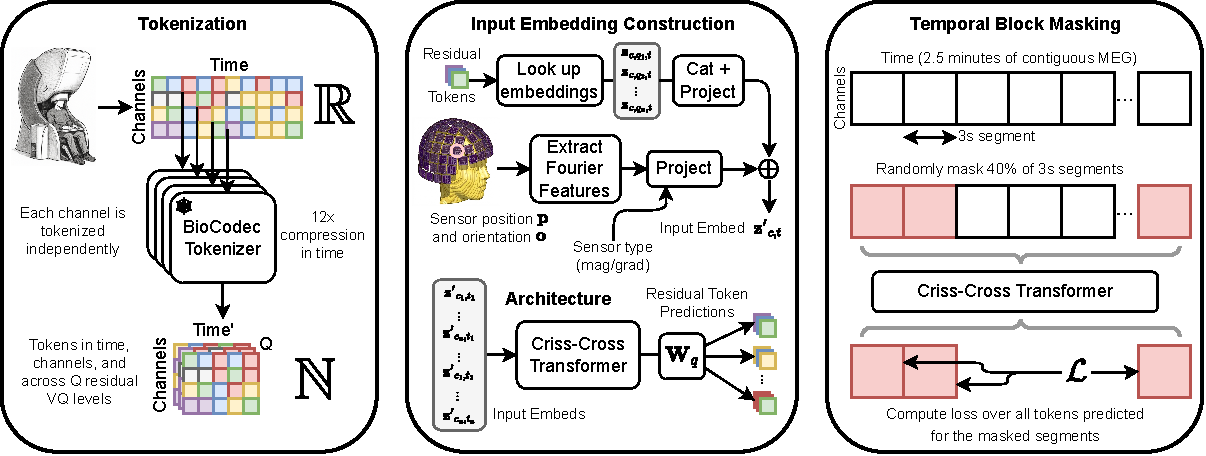
\includegraphics[width=0.98\linewidth,height=0.62\textheight,keepaspectratio]{imagenes/tlsmethod.pdf}\par
  \vspace{-1mm}
  \makebox[0.98\linewidth][r]{\tiny\color{muted}Fuente: MEG-XL}

  \vspace{2mm}

  \makebox[0.72\linewidth][c]{%
    \parbox[t]{0.20\linewidth}{\centering\smallmetric{150 s}{contexto}}%
    \hfill
    \parbox[t]{0.20\linewidth}{\centering\smallmetric{50}{bloques}}%
    \hfill
    \parbox[t]{0.20\linewidth}{\centering\smallmetric{20/50}{máscara}}%
  }

  \note{El mensaje clave: durante el preentrenamiento no se entrena a reconocer palabras. Se aprende una representación previa que después se ajusta a la tarea supervisada.}
\end{frame}

% 11 --------------------------------------------------------------------------
\begin{frame}[c]{Fine-tuning: recuperación contextual de palabras}
  \begin{columns}[c,totalwidth=\linewidth]
    \hspace*{0.05\linewidth}
    \begin{column}{0.40\linewidth}
      \begin{block}{Construcción del ejemplo}
        \begin{itemize}
          \item Cada palabra tiene un tiempo de inicio.
          \item Se extrae una ventana EEG de 3 s.
          \item 50 palabras forman una entrada de 150 s.s
        \end{itemize}
      \end{block}

      \begin{block}{Objetivo lingüístico}
        La representación cerebral se proyecta al espacio de embeddings de \textit{T5-large}.
      \end{block}
    \end{column}

    \begin{column}{0.51\linewidth}
      \centering
      \begin{tikzpicture}[node distance=4mm, every node/.style={font=\scriptsize}]
        \node[draw=deepgreen, fill=deepgreen!8, rounded corners, text width=42mm, align=center] (textgrid) {TextGrid: inicio de palabra};
        \node[draw=greenish, fill=greenish!12, rounded corners, text width=42mm, align=center, below=of textgrid] (win) {ventana EEG de 3 s};
        \node[draw=warning, fill=warning!18, rounded corners, text width=42mm, align=center, below=of win] (seq) {50 palabras $\rightarrow$ 150 s};
        \node[draw=accent, fill=accent!12, rounded corners, text width=42mm, align=center, below=of seq] (proj) {proyección a 1024 dimensiones};
        \node[draw=deepgreen, fill=deepgreen!8, rounded corners, text width=42mm, align=center, below=of proj] (rank) {ranking Top-10 por coseno};
        \foreach \x/\y in {textgrid/win,win/seq,seq/proj,proj/rank}{\draw[-{Latex[length=2mm]}, thick, deepgreen] (\x) -- (\y);}
      \end{tikzpicture}
    \end{column}
  \end{columns}

  \note{Explicar que la pregunta de evaluación no es generar texto, sino si la palabra correcta queda entre las 10 más parecidas dentro de un vocabulario cerrado.}
\end{frame}

% 12 --------------------------------------------------------------------------
\begin{frame}[c]{Diseño experimental: separar efectos}
  \small
  \renewcommand{\arraystretch}{1.22}
  \setlength{\tabcolsep}{5pt}
  \begin{center}
  \begin{tabular}{>{\bfseries}p{0.25\linewidth}p{0.22\linewidth}p{0.26\linewidth}p{0.18\linewidth}}
    \toprule
    Condición & Inicialización & Preentrenamiento EEG & Fine-tuning \\
    \midrule
    Sin preentrenamiento & Aleatoria & No & ds004408 \\
    EEG desde cero & Aleatoria & Lectura $\rightarrow$ escucha & ds004408 \\
    MEG-XL + emb. EEG & Checkpoint MEG-XL & Lectura $\rightarrow$ escucha & ds004408 \\
    MEG-XL + emb. MEG & Checkpoint MEG-XL & Lectura $\rightarrow$ escucha & ds004408 \\
    \bottomrule
  \end{tabular}
  \end{center}

  \vspace{3mm}

  \begin{block}{Qué permite medir}
    \begin{itemize}
      \item Efecto del preentrenamiento autosupervisado con EEG.
      \item Efecto de inicializar desde MEG-XL.
      \item Efecto de reutilizar o redefinir el embedding de tipo de sensor.
    \end{itemize}
  \end{block}

  \note{Esta diapositiva es importante metodológicamente. No hay que vender solo el mejor resultado: hay que explicar que las condiciones separan qué componente aporta la mejora.}
\end{frame}

% 13 --------------------------------------------------------------------------
\begin{frame}[c]{Resultado principal}
  \begin{columns}[c,totalwidth=\linewidth]
    \begin{column}{0.44\linewidth}
      \begin{block}{Métrica principal}
        Top-10 balanceada sobre las 250 palabras más frecuentes de ds004408.
      \end{block}

      \begin{center}
        \bigmetric{22,32\%}{mejor modelo: MEG-XL + embedding MEG}
        \bigmetric{4,00\%}{azar uniforme con 250 candidatos}
      \end{center}
    \end{column}

    \begin{column}{0.52\linewidth}
      \scriptsize
      \renewcommand{\arraystretch}{1.22}
      \setlength{\tabcolsep}{4pt}
      \begin{tabular}{>{\bfseries}p{0.44\linewidth}>{\centering\arraybackslash}p{0.20\linewidth}>{\centering\arraybackslash}p{0.23\linewidth}}
        \toprule
        Condición & Bal. 250 & Bal./azar \\
        \midrule
        Sin preentrenamiento & 4,05\% & 1,01 \\
        EEG desde cero & 19,95\% & 4,99 \\
        MEG-XL + emb. EEG & 20,56\% & 5,14 \\
        MEG-XL + emb. MEG & \textbf{22,32\%} & \textbf{5,58} \\
        \bottomrule
      \end{tabular}

      \vspace{3mm}

      \begin{exampleblock}{Lectura rápida}
        La mejora dominante viene del preentrenamiento EEG; la transferencia desde MEG-XL añade una ganancia menor pero positiva.
      \end{exampleblock}
    \end{column}
  \end{columns}

  \note{Primero leer el azar y el mejor resultado. Después explicar la comparación por filas: sin preentrenamiento no aprende, EEG desde cero da el salto principal, MEG-XL mejora algo más.}
\end{frame}

% 14 --------------------------------------------------------------------------
\begin{frame}[c]{Dinámica de validación}
  \begin{columns}[c,totalwidth=\linewidth]
    \begin{column}{0.58\linewidth}
      \centering
      \IfFileExists{../memoria/figuras/fig_5_2_ds004408_val_balanced_top10_250.pdf}{%
        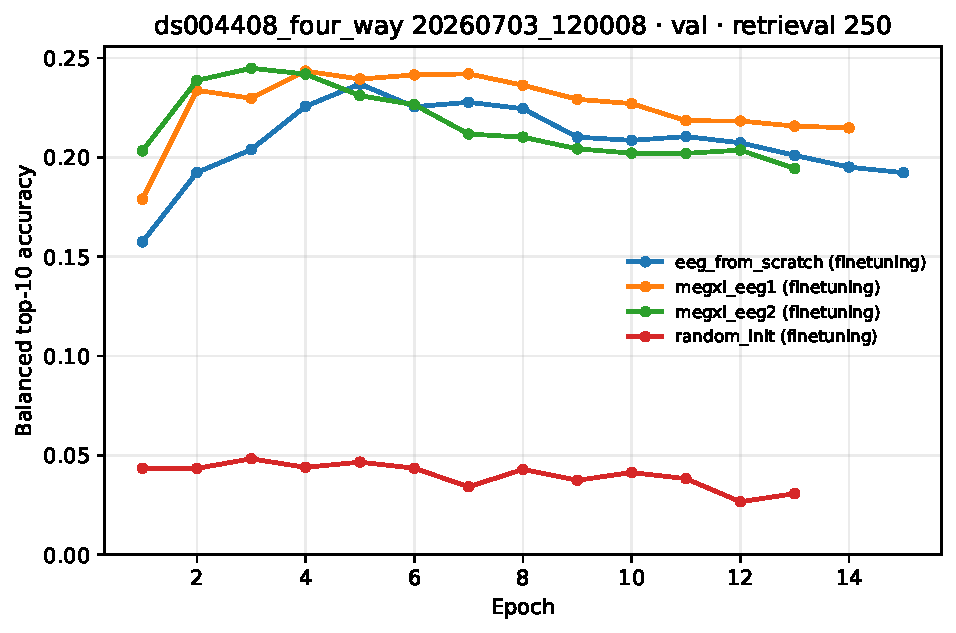
\includegraphics[width=\linewidth,height=0.62\textheight,keepaspectratio]{../memoria/figuras/fig_5_2_ds004408_val_balanced_top10_250.pdf}%
      }{%
        \begin{tikzpicture}[x=.75cm,y=.55cm]
          \draw[->, thick] (0,0) -- (6.8,0) node[right]{épocas};
          \draw[->, thick] (0,0) -- (0,4.5) node[above]{validación};
          \draw[accent, thick] plot[smooth] coordinates {(0,0.8)(1,0.9)(2,0.8)(3,0.85)(4,0.82)(5,0.78)};
          \draw[warning, thick] plot[smooth] coordinates {(0,2.0)(1,2.6)(2,3.0)(3,3.2)(4,3.1)(5,2.8)};
          \draw[deepgreen, thick] plot[smooth] coordinates {(0,2.3)(1,3.0)(2,3.6)(3,3.9)(4,3.5)(5,3.1)};
          \node[font=\scriptsize] at (3.3,-0.7) {máximo temprano};
        \end{tikzpicture}%
      }
    \end{column}

    \begin{column}{0.38\linewidth}
      \begin{block}{Observación}
        Los mejores checkpoints aparecen en pocas épocas.
      \end{block}

      \begin{alertblock}{Riesgo}
        Continuar el fine-tuning no mejora necesariamente y puede degradar la generalización.
      \end{alertblock}

      \begin{exampleblock}{Interpretación}
        El preentrenamiento proporciona una representación útil, pero el EEG se sobreajusta con facilidad.
      \end{exampleblock}
    \end{column}
  \end{columns}

  \note{No entrar en todos los detalles de la gráfica. El mensaje es que la ganancia se obtiene pronto y que el ajuste supervisado prolongado puede ser perjudicial.}
\end{frame}

% 15 --------------------------------------------------------------------------
\begin{frame}[c]{Interpretación de los resultados}
  \small
  \begin{columns}[T,totalwidth=\linewidth]
    \begin{column}{0.30\linewidth}
      \begin{block}{Viabilidad}
        \begin{minipage}[t][30mm][t]{\linewidth}
        \begin{itemize}
          \item La arquitectura puede adaptarse a EEG.
          \item El sistema queda claramente por encima del azar.
          \item El contexto largo es compatible con la tarea.
        \end{itemize}
        \end{minipage}
      \end{block}
    \end{column}
    \hfill

    \begin{column}{0.30\linewidth}
      \begin{block}{Qué aporta más}
        \begin{minipage}[t][30mm][t]{\linewidth}
        \begin{itemize}
          \item El mayor salto viene del preentrenamiento EEG.
          \item MEG-XL aporta una mejora adicional moderada.
          \item El embedding MEG reutilizado fue el mejor en esta ejecución.
        \end{itemize}
        \end{minipage}
      \end{block}
    \end{column}
    \hfill

    \begin{column}{0.30\linewidth}
      \begin{alertblock}{Prudencia}
        \begin{minipage}[t][30mm][t]{\linewidth}
        \begin{itemize}
          \item Una única semilla.
          \item Protocolos no idénticos a todos los trabajos previos.
          \item No es generación libre de texto.
        \end{itemize}
        \end{minipage}
      \end{alertblock}
    \end{column}
  \end{columns}

  \vspace{3mm}

  \begin{center}
    \begin{tikzpicture}
      \node[draw=deepgreen, fill=soft, rounded corners=3pt, inner xsep=8pt, inner ysep=4pt, text width=0.86\linewidth, align=center]{
        \textbf{Lectura honesta:} la transferencia MEG--EEG no resuelve el brain-to-text no invasivo, pero muestra una vía viable y medible para avanzar.
      };
    \end{tikzpicture}
  \end{center}

  \note{Esta diapositiva debe sonar madura: buen resultado, pero sin venderlo como una superioridad definitiva.}
\end{frame}

% 17 --------------------------------------------------------------------------
\begin{frame}[c]{Conclusiones}
  \small
  \begin{columns}[T,totalwidth=\linewidth]
    \begin{column}{0.30\linewidth}
      \begin{block}{Qué se ha conseguido}
        \begin{minipage}[t][30mm][t]{\linewidth}
        \begin{itemize}
          \item Adaptar MEG-XL a EEG heterogéneo.
          \item Entrenar con lectura y escucha.
          \item Evaluar recuperación de palabras en ds004408.
        \end{itemize}
        \end{minipage}
      \end{block}
    \end{column}
    \hfill

    \begin{column}{0.30\linewidth}
      \begin{block}{Resultado central}
        \begin{minipage}[t][30mm][t]{\linewidth}
        \begin{itemize}
          \item 22,32\% Top-10 balanceada.
          \item 5,58 veces el azar.
          \item El preentrenamiento EEG es decisivo.
        \end{itemize}
        \end{minipage}
      \end{block}
    \end{column}
    \hfill

    \begin{column}{0.30\linewidth}
      \begin{block}{Trabajo futuro}
        \begin{minipage}[t][30mm][t]{\linewidth}
        \begin{itemize}
          \item Más semillas y particiones.
          \item Más bandas, tokenizadores y datasets.
          \item Registros propios con casco EEG.
        \end{itemize}
        \end{minipage}
      \end{block}
    \end{column}
  \end{columns}

  \vspace{3mm}

  \begin{center}
    \begin{tikzpicture}
      \node[draw=deepgreen, fill=soft, rounded corners=3pt, inner xsep=8pt, inner ysep=4pt, text width=0.86\linewidth, align=center]{
        \textbf{Conclusión final:} una arquitectura de contexto largo inspirada en MEG-XL puede adaptarse a EEG y obtener resultados competitivos en una tarea controlada de clasificación contextual de palabras.
      };
    \end{tikzpicture}
  \end{center}

  \note{Cerrar con tres ideas: viable, por encima de azar, falta confirmar con más experimentación.}
\end{frame}

% 18 --------------------------------------------------------------------------

{
\setbeamercolor{background canvas}{bg=deepgreen}
\begin{frame}
  \begin{columns}[c,totalwidth=\linewidth]
    \begin{column}{0.43\linewidth}
      \centering
      {\Huge\bfseries\color{white}Gracias\par}
      \vspace{7mm}
      {\Large\color{white}Preguntas\par}
    \end{column}

    \begin{column}{0.52\linewidth}
      \centering
      
\includegraphics[width=\linewidth,height=0.78\textheight,keepaspectratio]{imagenes/luffy_transparent_2.png}
    \end{column}
  \end{columns}
\end{frame}
}

\end{document}
